\documentclass{article}

\usepackage{hyperref}
\usepackage{tabularx}
\usepackage[explicit]{titlesec}
\usepackage{fullpage}
\usepackage{titling}
\usepackage{graphicx}
\usepackage{float}
\usepackage{color}
\usepackage{booktabs}

\setlength{\droptitle}{-14ex}  

\titleformat{\section}
  {\normalfont\large\bfseries}{\thesection}{1em}{{#1}}

\titleformat{\subsection}
  {\normalfont\bfseries}{\thesection}{1em}{{#1}}

\title{CAS 741: Problem Statement\\[10pt]\Large Dynamical Systems: 
Multi-Pendulum Simulation (MPSim)}

\author{Karol Serkis\\\texttt{serkiskj@mcmaster.ca}}

\date{}

%% Comments

\usepackage{color}

\newif\ifcomments\commentsfalse

\ifcomments
\newcommand{\authornote}[3]{\textcolor{#1}{[#3 ---#2]}}
\newcommand{\todo}[1]{\textcolor{red}{[TODO: #1]}}
\else
\newcommand{\authornote}[3]{}
\newcommand{\todo}[1]{}
\fi

\newcommand{\wss}[1]{\authornote{blue}{SS}{#1}}
\newcommand{\spc}[1]{\authornote{magenta}{SP}{#1}}

\begin{document}

%\pagenumbering{gobble}
\pagenumbering{alph}

\maketitle

\begin{table}[hp]
\caption{Revision History} \label{TblRevisionHistory}
\begin{tabularx}{\textwidth}{llX}
\toprule
\textbf{Date} & \textbf{Developer(s)} & \textbf{Change}\\
\midrule
September 17, 2018 & Karol Serkis & First revision of document\\
September 14, 2018 & Karol Serkis & Problem Idea proposed \& discussed with Dr.
Spencer Smith \\
December 18, 2018 & Karol Serkis & Problem Statement \& bibliography fixed, 
\& program name fixed \\
\bottomrule
\end{tabularx}
\end{table}

\section*{Problem}

A simple gravity pendulum has very easy to system to model and consists of a
weight suspended from a pivot and the weight is given enough space to swing
freely. To simplify the model we assume no air resistance and a friction-less
pivot~\cite{WikiPendulum}. The model and calculations for the simple gravity 
pendulum are well defined and only require ordinary differential equation (ODE) 
solvers as well as Lagrangian mechanics equations~\cite{MathPendulum}. Below
is an example of a single pendulum to demonstrate the idea:
\begin{figure}[H]
	\centering
	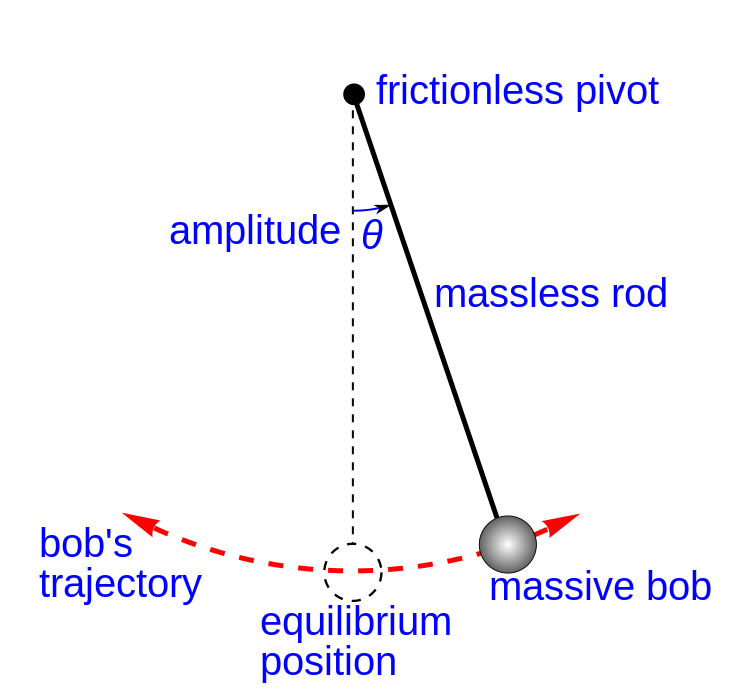
\includegraphics[width=250px]{simple-pend.png}
\caption{A simple gravity pendulum: friction-less pivot \& no air 
resistance~\cite{WikiPendulum}}
	\label{fig:simplepend}
\end{figure}

However, once you attach a pendulum to the bottom of another pendulum in the
case of a double pendulum you have a new system that is dynamic and chaotic and
requires a set of coupled ordinary differential equation 
solvers~\cite{DoublePendulum}. Once you introduce multiple pendulums the system 
becomes chaotic and interesting to model and simulate.

\begin{figure}[h]
	\centering
	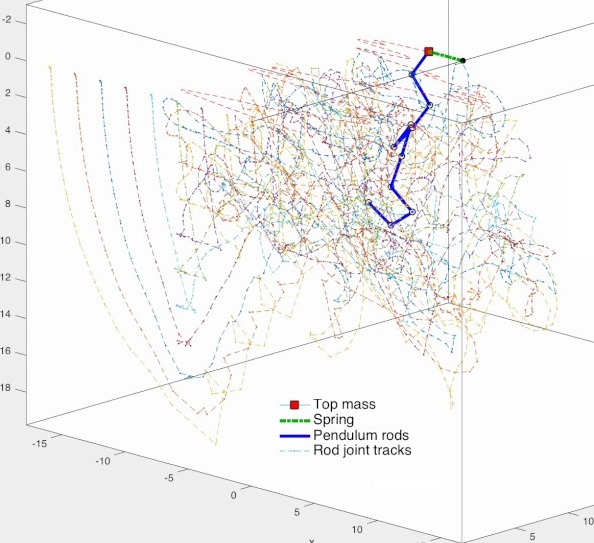
\includegraphics[width=220px]{multi-pend.jpg}
	\caption{An example of dynamical and chaotic system with
	Spring-Mass-Multi-Pendulum~\cite{MLSim}}
	\label{fig:multipend}
\end{figure}

\section*{Proposed Solution}
A proposed software solution will produce a simulation of a multi-pendulum
system. Inspiration for this problem came from Dr. Ned Nedialkov's Multi-body
Lagrangian Simulations using DAETS (Differential-Algebraic Equations by Taylor
Series). DAETS is a C++ package for solving initial value problems for DAE
systems~\cite{DAETS}.

\begin{figure}[h]
	\centering
	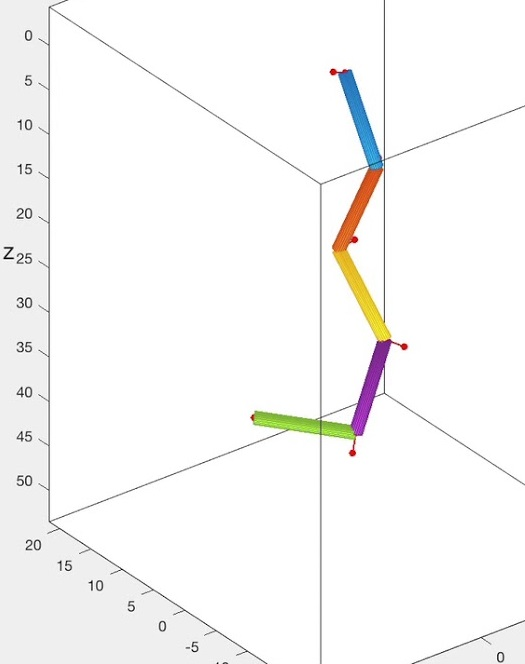
\includegraphics[width=150px]{3pend.jpg}
	\caption{Simulation of Multi-Pendulum system using 
	DAETS~\cite{MLSim}}
	\label{fig:simpendula}
\end{figure}

The proposed software is to develop a multi-platform equivalent solution that
only focuses on multi-pendulum simulations and tracking the chaotic motion of
the system. It will allow users to track kinetic and potential energy over time 
using ODE/DAE initial value problem solvers, and display a simulation showing
the animated trajectory of the pendulums~\cite{DAETS}. To make things simpler
to animate and calculate we can restrict to a rigid-body system, where the mass 
of each pendulum rod is located at the center of gravity of each 
rod~\cite{DoublePendulum}.

\begin{figure}[!htb]
	\centering
	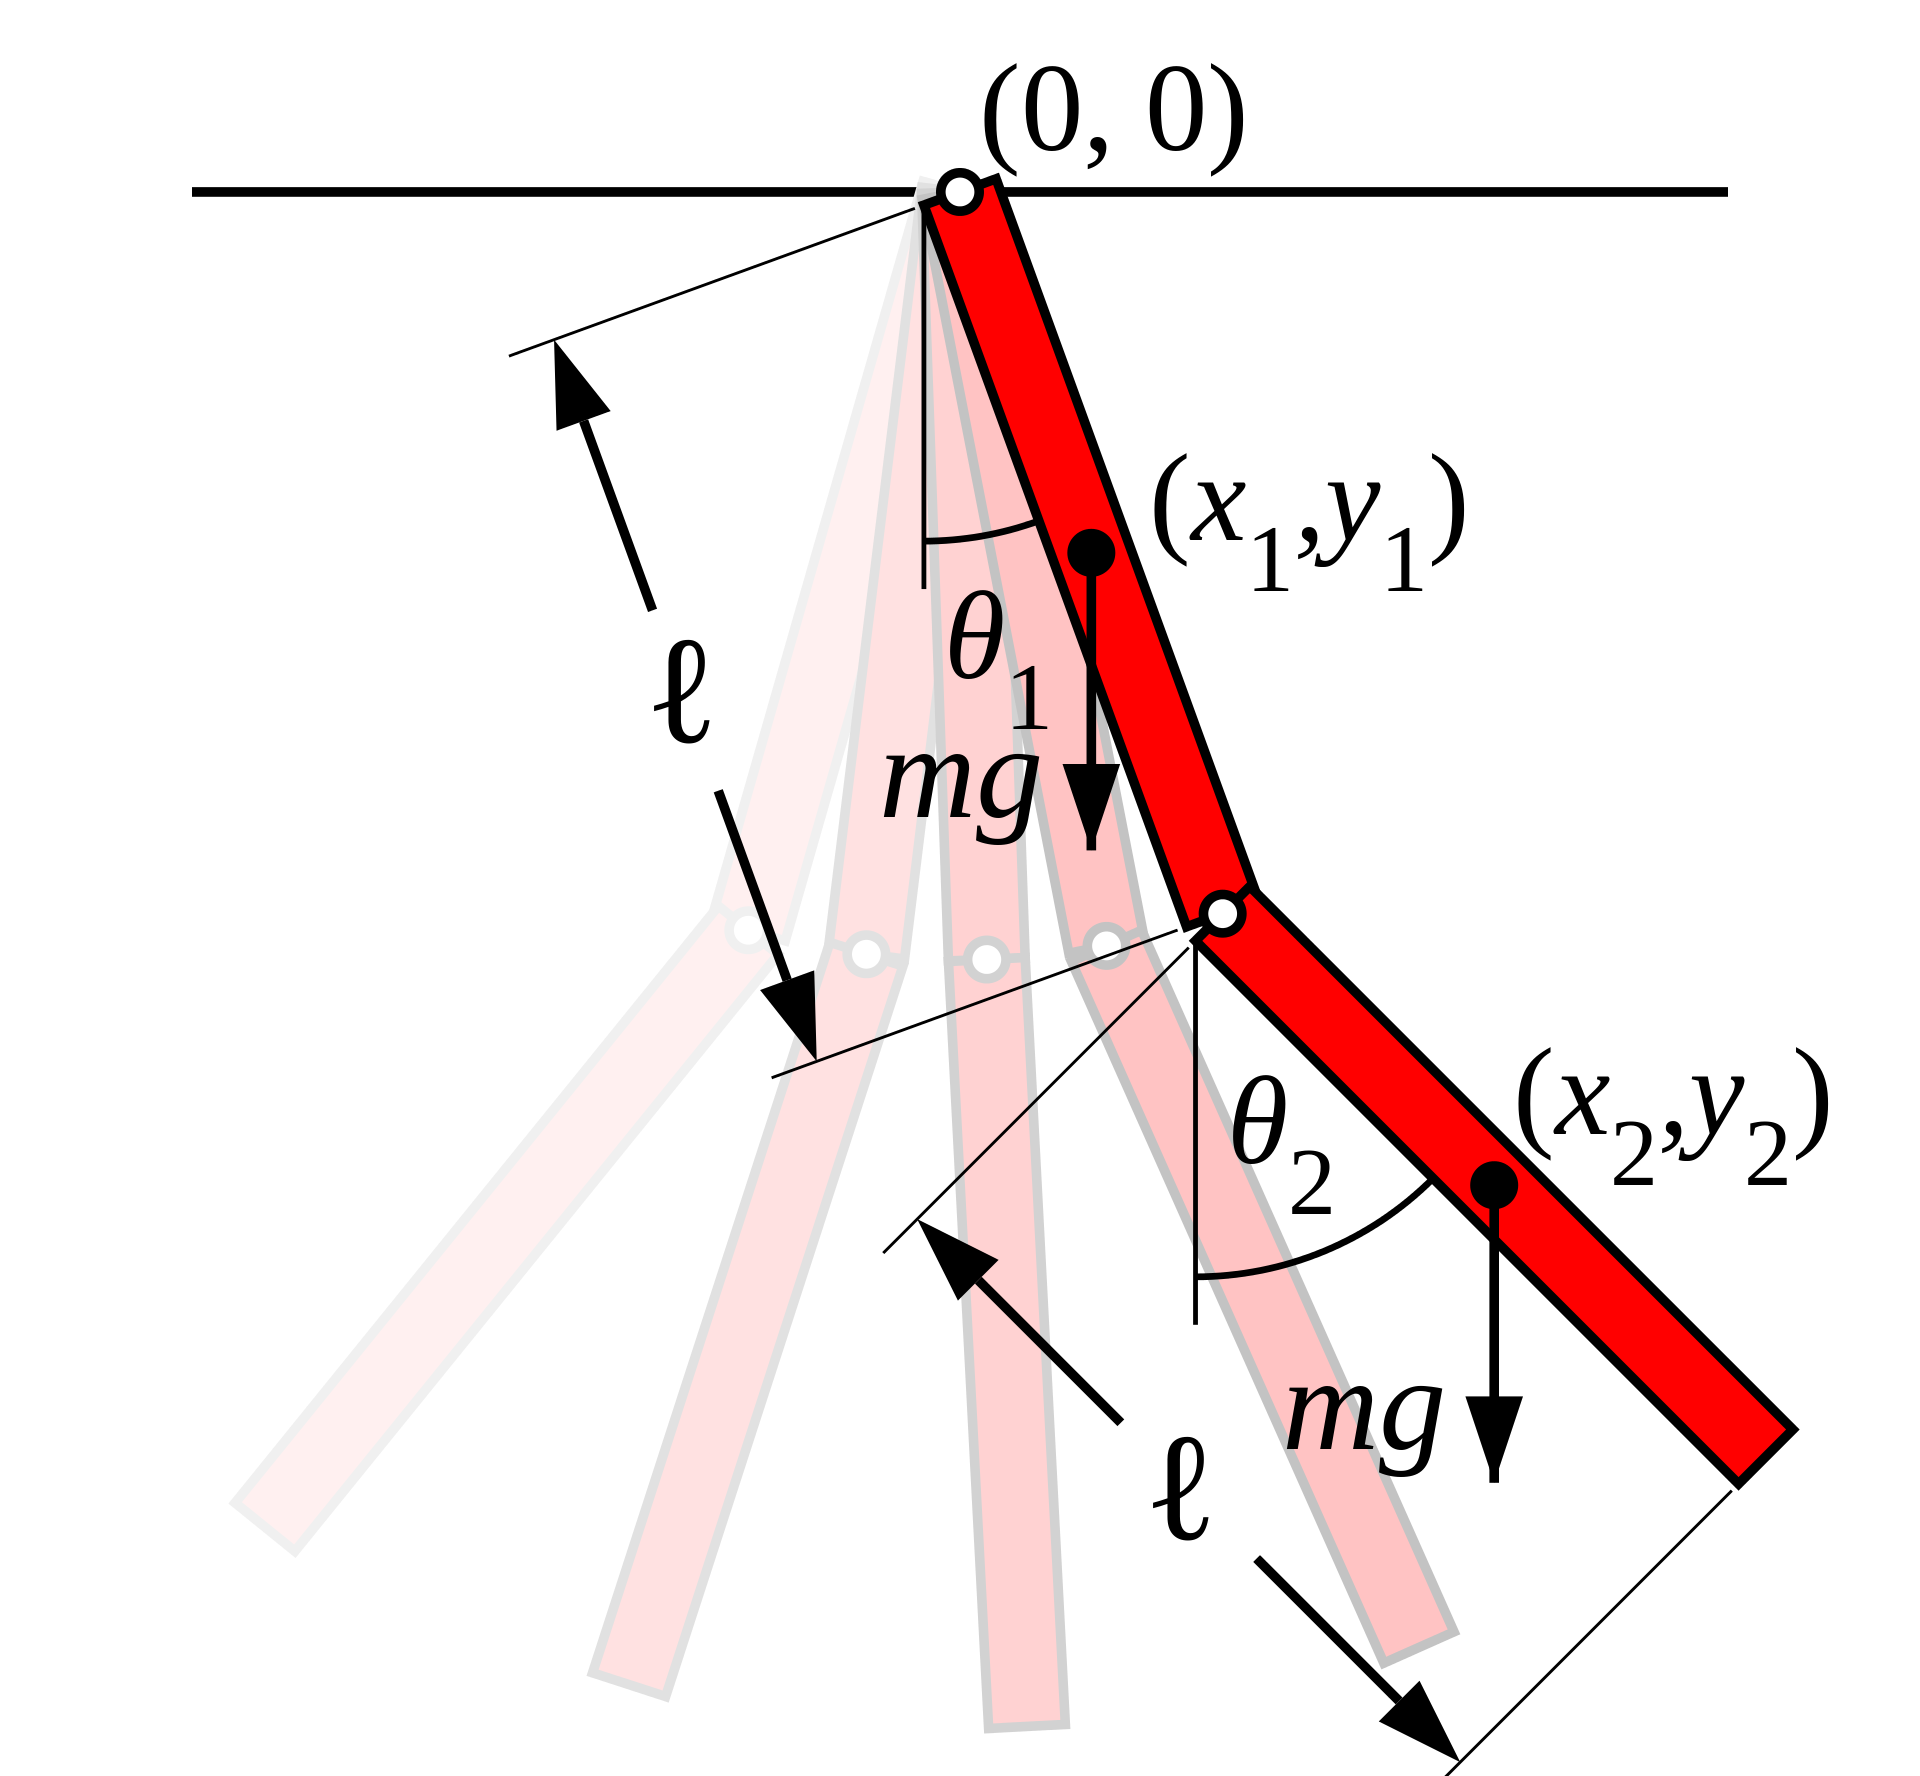
\includegraphics[width=220px]{Double-pendulum-rigid.png}
	\caption{An example of rigid-body double 
	pendulum~\cite{DoublePendulum}}
	\label{fig:multipend}
\end{figure}

\section*{Context}
\subsection*{Environment}
The simulation software will be created with multi-platform support in mind and
be compatible with Windows 10, Mac OS, Linux, etc. In order to achieve this,
Python will be used for development and implementation of the simulation
software.

\subsection*{Stakeholders}
Specific stakeholders include:
\begin{itemize}
\item Karol Serkis
\item Dr. Spencer Smith
\item Dr. Ned Nedialov
\item Students of CAS 741 
\item Individuals studying or working in fields related to physics
\end{itemize}

\newpage
\begin{thebibliography}{9}
\bibitem{WikiPendulum} 
Wikipedia - Pendulum, \\\url{https://en.wikipedia.org/wiki/Pendulum}

\bibitem{MathPendulum} 
Wikipedia - Pendulum (mathematics), 
\\\url{https://en.wikipedia.org/wiki/Pendulum_(mathematics)}

\bibitem{DoublePendulum} 
Wikipedia - Double Pendulum, 
\\\url{https://en.wikipedia.org/wiki/Double_pendulum}

\bibitem{DAETS} 
Differential-Algebraic Equations by Taylor Series, 
\\\url{http://www.cas.mcmaster.ca/~nedialk/daets/}

\bibitem{MLSim} 
Multi-body Lagrangian Simulations, 
\\\url{https://www.youtube.com/channel/UCCuLchOx0W0yoNE9KOCYlVQ}

\end{thebibliography}

\end{document}
